\section{Development methods}

\paragraph{Classic software design approach}

In every software development project, a visual sketch of the system is often created in order to aid the design process, and act as a visual guide during the documentation. However, implementing whatever design created earlier is not always trivial. The primary and most widespread embedded programming language, the \verb!C!, has been designed as a "Professional Programmers Language"\cite{essentialc}, and it supports only very basic syntax checks, but nothing ensures that the program will behave as the programmer intended. The designer must choose to take the risks of unexpected errors, or a thorough testing must be conducted in order to ensure the correct and reliable functioning of the system. While the testing of simple systems can be finished quickly, dangers arise when the same method is used in a large multi-developer project. Most of the industry have responded to this by scaling up the work force that gave birth to a number of strict project safety standards, internal regulations and coding guidelines\cite{misra}, and led to a huge amount of overhead in human labour in each software development project.

\paragraph{Model Based Design}

As described earlier, the Model based design is based on solving the problems in a more visual environment. During the development, there is  limited connection between the designed software and the target hardware. Many of the solutions can be verified using the simulated model of the system, resulting in an accelerated development process\cite{locomotive}.
Due to the heavy reliance on abstract models and their connections, even if significant changes occur in the specifications, only minimal amount of modification is required to the code that formulates the final software. This advantage can not be over emphasized, because the final specifications of the system are rarely known, especially in prototype development.
Although it has its own limitations as well, model based design relies on complex tools to do most of the work, and their operation and integration into an existing project is difficult and become less practical or limited because of the lack of sufficient support as well.

\paragraph{Background}

For the \textbf{RobonAUT 2014} contest, we used \verb!MATLAB! and \verb!Simulink! to implement the control system and the state machine. We chose the \verb!MathWorks! product family, because \verb!Simulink! has extensive support for model and simulation based development, and allows the generation of \verb!C! source code that can be later used on any hardware that is capable of running \verb!FreeRTOS! or any other hard real-time operating systems. We have have used these technologies before successfully in industrial environment, which allowed us to follow out the concept.

\section{Model based design of the system}

% Contributions

Figure \ref{fig:architecture} shows the basic system connections and stages of deployment. A typical system designed in \verb!MATLAB! can be divided to the following parts.

\begin{enumerate}
\item A \verb!MATLAB! \verb!Script! that defines the system model and computes the simulator and controller parameters.
\item Based on these parameters we can build the simulator and control software in \verb!Simulink! that interact with each other.
\item If the system response in the simulation is correct, the controller is ready for code generation and field-testing.
\item The generated source code is invoked by the core operating system, the \verb!FreeRTOS! in this case
\item All communication with the hardware in implemented by the Core.
\end{enumerate}

\begin{figure}[!ht]
    \centering
    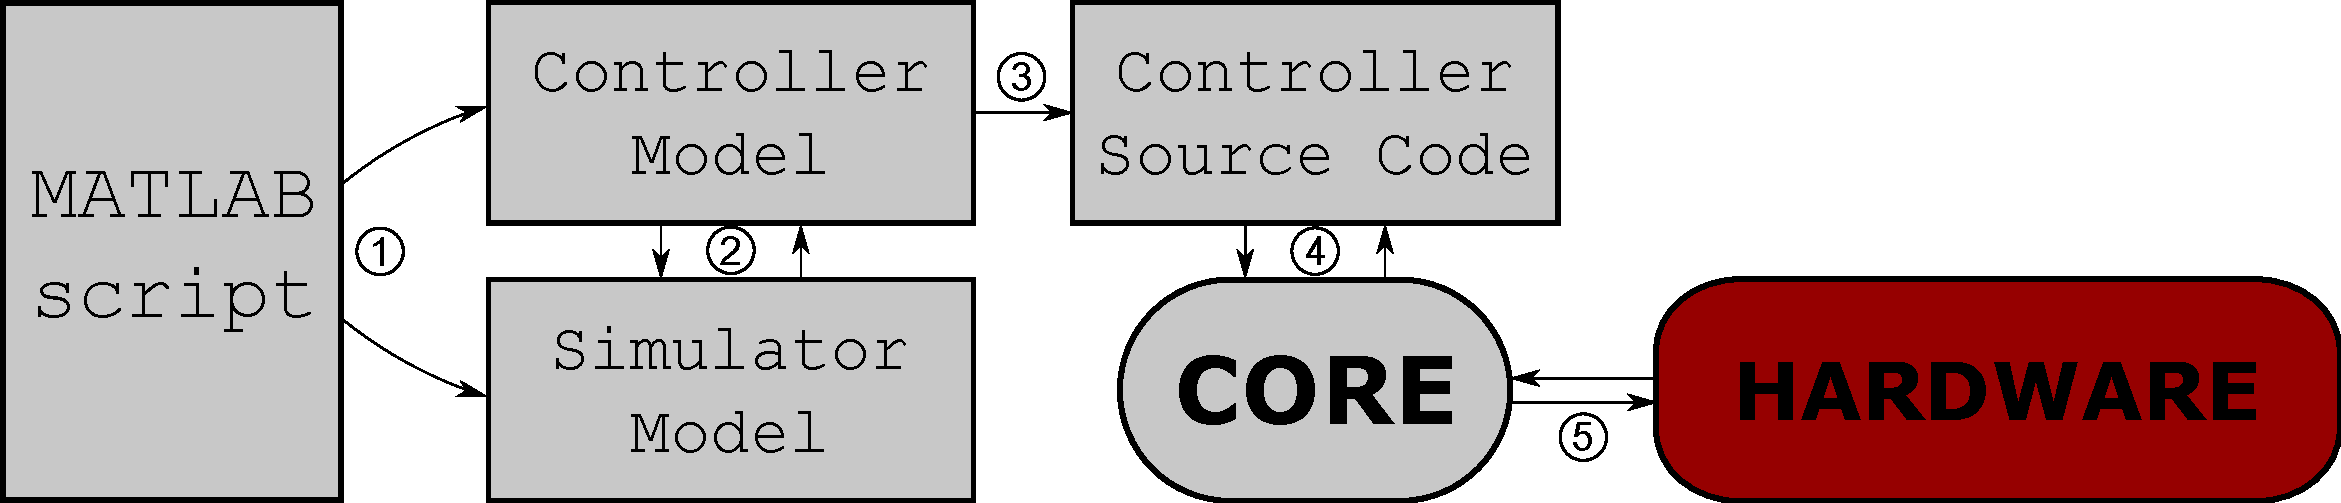
\includegraphics[width=0.7\linewidth]{img/architecture}
    \caption{Connections and dependencies}
    \label{fig:architecture}
\end{figure}

Although in most cases the core unit of a complex software will be an operating system, it is not mandatory. Therefore we use the \emph{Core} expression in this paper, but it refers to the FreeRTOS operating system in our case.

\subsection{Functional description}

During the race, the track is marked by a dark line on light ground. The car follows this trail that guides it through certain checkpoints. In between there are obstacles that need to be passed in a specific way. Each obstacle is marked in a unique manner that allows the car to unambiguously determine, based on simple on-board sensors, which function it has to execute in the current segment.

The recommended sensor outfit\cite{sensors} is a number of optoelectronic sensors beneath the front axis or bumper of the car, and a couple of infrared proximity sensors at the front and two sides of the car. Certain teams extended this setup with a camera for image-recognition, a second optosensor array or ultrasound proximity sensors, but this paper will not consider any of these layouts.

\subsection{Building a model}

The first step in model based design is to create a model of the system, based on the functional description and known sensor fitting. To follow the line, the signals of the optical array must be processed and a control system must use this input to keep the car on the track. Let's define the following state variables:

\begin{center}
  \begin{tabular}{| c | p{0.7\linewidth} |}
\hline
    d & Position error: The shortest distance between the centre of the front optical array and the centre of the track \\ \hline
    $ \delta $ & Angular error: The angle between the centreline of the body and the tangent of the track \\ \hline
    $ \Phi $ & Steering angle: The effective steering angle, according to Ackermann-steering \\
    \hline
    $ \kappa $ & Current curvature of the track ($1/R$) \\ \hline
    x & Line position: the position of the track line along the front optical array \\ \hline
    c & Line speed: derivative of x, the change of the track line position \\ \hline
    v & Car speed: The current speed of the car along the centreline \\
    \hline
  \end{tabular}
\end{center}

Other variables with temporary significance might be defined in the text before their usage. Figure \ref{fig:cartop} helps to visualize the basic geometrics of the car, and the connections of the state variables.

\begin{figure}[!ht]
    \centering
    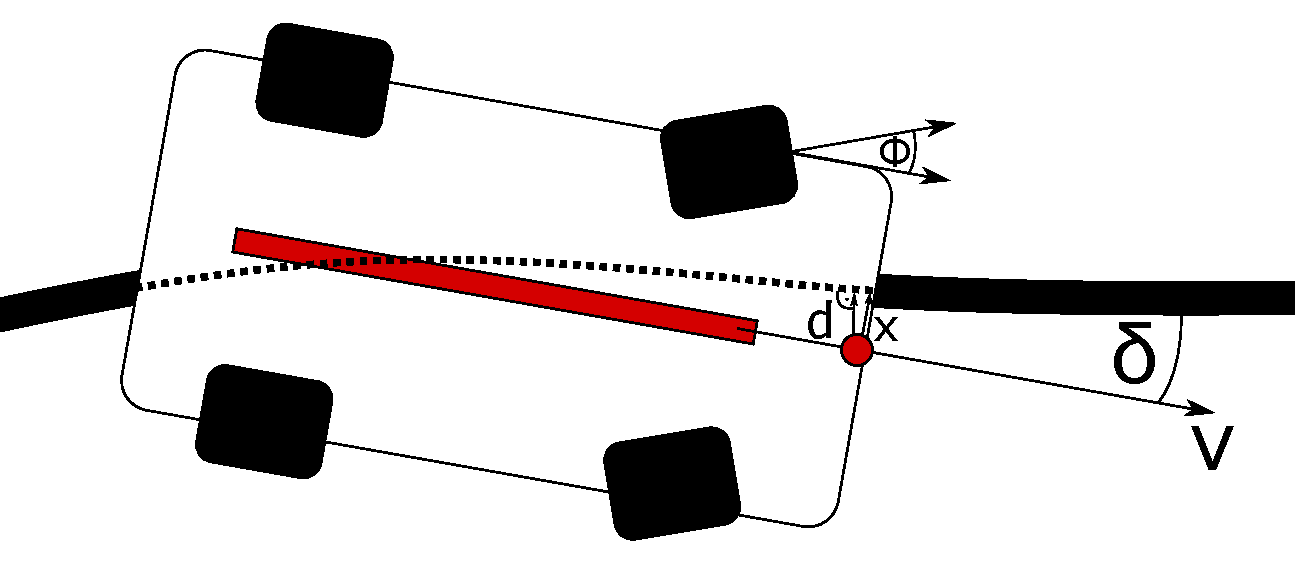
\includegraphics[width=0.7\linewidth]{img/cartop}
    \caption{System model}
    \label{fig:cartop}
\end{figure}

\paragraph{Formulating the system model}

Knowing the dynamical system equations~(\ref{eq:of1}, \ref{eq:of2}), and parameters (L: wheelbase), we can formulate the \textbf{A} and \textbf{B}\footnote{The system is in discrete-time, but the continuous-time notation will be used throughout the paper, for better readability.} matrices based on their linear approximations in an equilibrium state $(d = 0; \delta = 0; v = 1)$ ~(\ref{eq:of3}).

\begin{align} 
    \dot{d} &= sin(\delta + \Phi) \cdot v  \label{eq:of1} \\ 
    \dot{\delta} &= \frac{v}{L} \cdot tan(\Phi) + \kappa \label{eq:of2}
\end{align}

% \begin{minipage}{0.45\linewidth}
%     \begin{align} \label{eq:of3}
%         \begin{bmatrix}
%                \dot{d} \\
%                \dot{\delta}
%         \end{bmatrix}
%         =
%         \begin{bmatrix}
%                0 & \delta \cdot v \\
%                0 & 0
%         \end{bmatrix}
%         %\cdot
%         \begin{bmatrix}
%                d \\
%                \delta
%         \end{bmatrix}
%      \end{align}
% \end{minipage}
% \begin{minipage}{0.45\linewidth}
%     \begin{align} \label{eq:of4}
%         \begin{bmatrix}
%                \dot{d} \\
%                \dot{\delta}
%         \end{bmatrix}
%         =
%         \begin{bmatrix}
%            0 & 0 \\
%            \frac{v}{L} & 1
%          \end{bmatrix}
%         %\cdot
%          \begin{bmatrix}
%                \Phi \\
%                \kappa
%         \end{bmatrix}
%      \end{align}
% \end{minipage}

    \begin{align} \label{eq:of3}
        \begin{bmatrix}
               \dot{d} \\
               \dot{\delta}
        \end{bmatrix}
        =
        \begin{bmatrix}
               0 & \delta \cdot v \\
               0 & 0
        \end{bmatrix}
        %\cdot
        \begin{bmatrix}
               d \\
               \delta
        \end{bmatrix}
		+
        \begin{bmatrix}
           0 & 0 \\
           \frac{v}{L} & 1
         \end{bmatrix}
        %\cdot
         \begin{bmatrix}
               \Phi \\
               \kappa
        \end{bmatrix}
     \end{align}

Instead of hard-coding the system matrices into the script, we can apply a different method that is nicer for the model based approach, by using the \verb!MATLAB! \verb!Symbolic! \verb!Toolbox!. This package allows the automatic generation of the Jacobi-matrices of the system, so the inputs are narrowed down to the system parameters and non-linear dynamic equations.
Furthermore, this way we can hold on to a lot more information that can later be used to generate a non-linear state observer, Extended Kalman Filter\cite{ekf}, or Hybrid Controller\cite{hybrid} for additional features in a complex system.
     


\paragraph{Control system}

Once an accurate system model is available, it's possible to formulate a controller. It's relatively easy to implement multiple controllers and compare them on the simulated system to determine, which would fit the robot the best.
Already knowing the state-space form of the system, a full-state feedback controller can be formulated quickly to stabilize the system. Using the Ackermann formula, we can obtain a suitable feedback matrix \textbf{K}, thus creating a stable new system with the feedback.

\begin{align}
	\underline{\dot{x}} = (A - BK) \cdot \underline{x}
\end{align}

\paragraph{Direct and inverse measurement models}

Unfortunately, a full-state feedback loop can rarely be realized directly, hence the controller we have just created would not be able to control the actual system. Certain states can not be measured but only estimated by a state observer. The controller must be prepared to do that. Simulating the sensor readings based on the state variables is possible with the \emph{Direct measurement model}, while in order to estimate the states based on the sensor readings we need the \emph{Inverse measurement model}.

Knowing the geometrical layout of the car, the expected signals can be simulated using inverse geometric projection to the optosensor array:

\begin{align}
    x = \frac{d}{\cos(\delta)}
\end{align}

After the direct model has been determined, the inverse model can be formulated as well:

\begin{align}
    \hat{d} &= x \cdot \cos(\delta) \\
    \hat{c} &=\dot{x} \\
    \hat{\delta} &= \arctan \left(\frac{c}{v}\right) - \Phi
\end{align}

The direct model is usually part of the simulation only, however, it is possible to proof-check the sensor readings during run-time. This can be especially useful, if the states are estimated by sensor fusion. The inverse measurement model is always the first layer of the control loop, and it is rarely found in the simulated environment.

Note: $\delta$ can be directly measured if the robot is equipped with multiple optosensor arrays, but of course a different inverse measurement model is still necessary.

\subsection{Building the simulation environment}

When the system model and controller are available, it is time to build the simulation environment. In case of a simple system, at this point the controller could be implemented directly in \verb!C!, but if the system is more complex, it is better practice to follow through the model based design. To test the behaviour of the system, the controller and the simulator must be implemented in \verb!Simulink! as well. Figure \ref{fig:simenvironment} shows the simulation based development concept. Because the Controller model and the Controller source code are identical, the key is to design a simulator that is deceptively similar to the real system, from the point of view of the controller. This is the reason why Direct and Inverse Measurement (msment) models are required.

\begin{figure}[!ht]
    \centering
    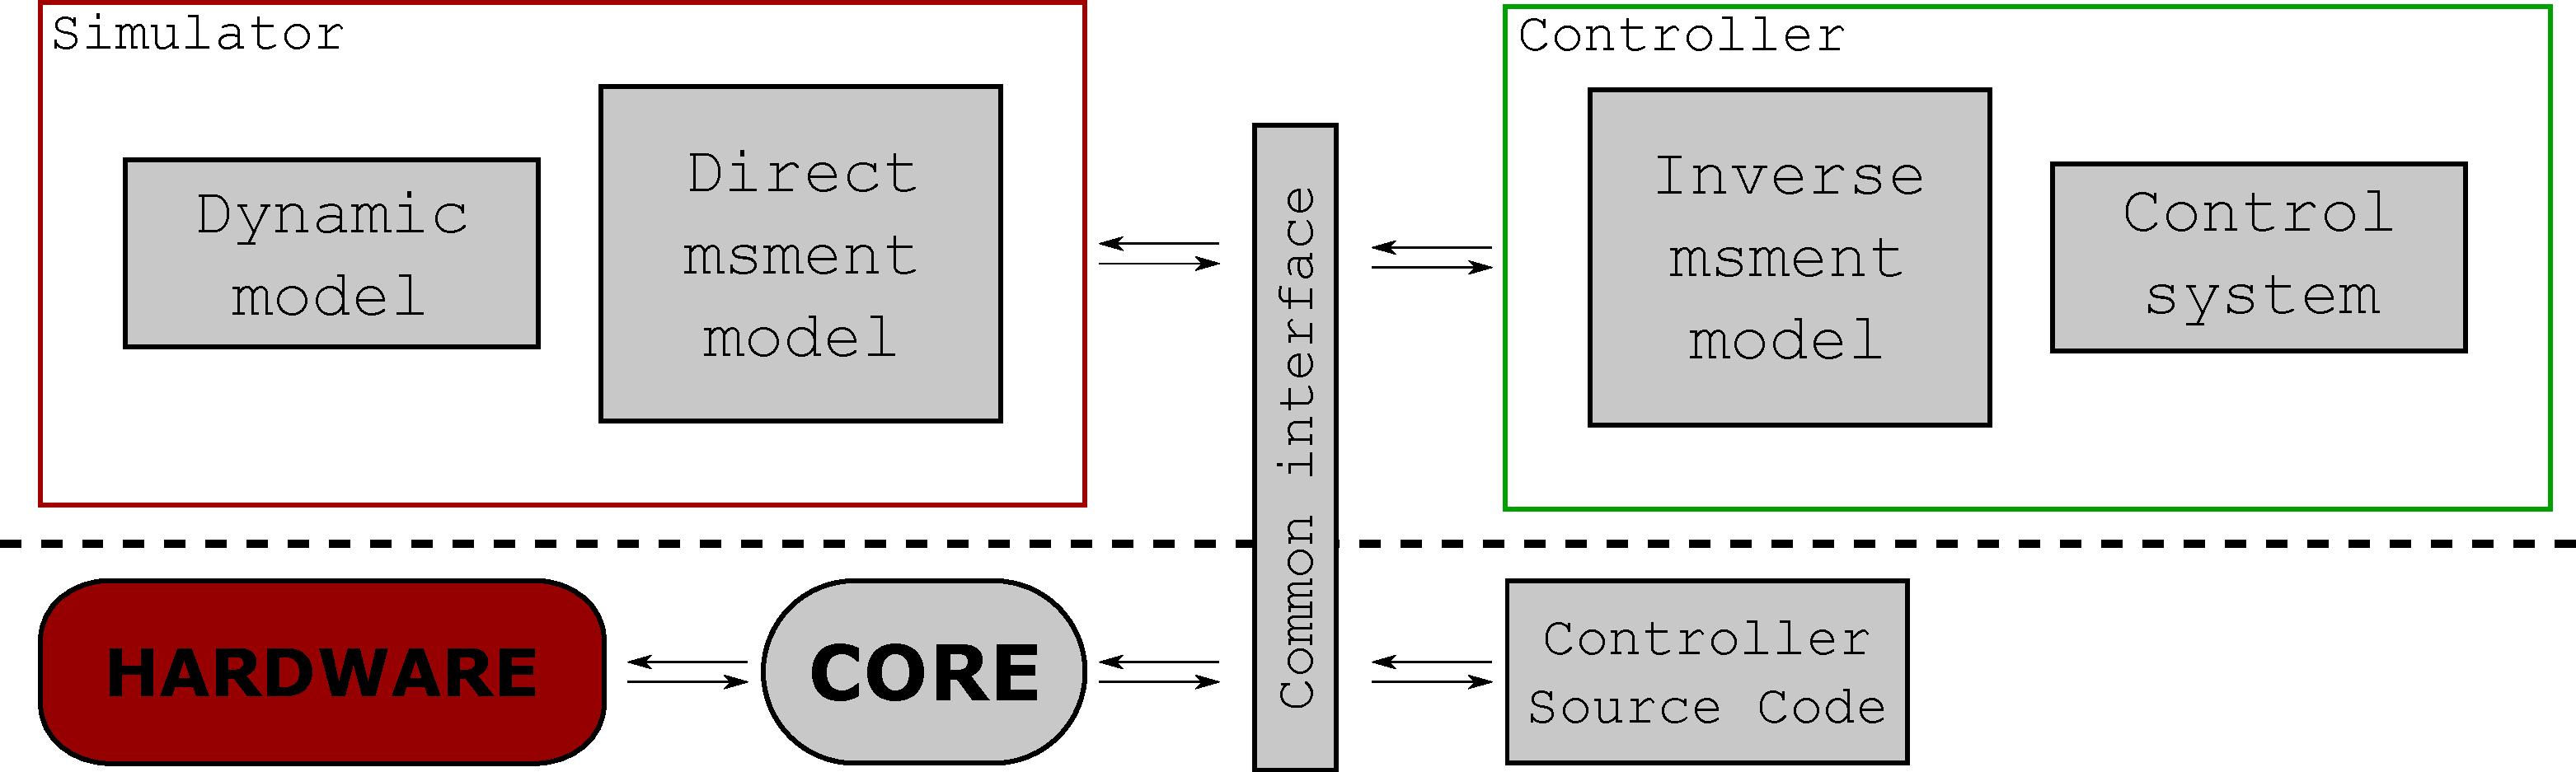
\includegraphics[width=0.7\linewidth]{img/simenvironment}
    \centering
    \caption{Simulation environment and analogy of deployment}
    \label{fig:simenvironment}
\end{figure}

Between the Simulator and Controller model, and between the Core and the Controller Source Code the actual sensor signals travel through a common interface, in the same form. The modules are interchangeable, without any functional loss. The modules themselves in the inside are working with the real (and estimated) state variables. The measurement models are mere encoding and decoding interfaces.

%Although \verb!MATLAB! is a dynamic typing language, it is good practice to fix the data type of the signals, especially if the software is developed for an embedded system. The default signal type is \emph{Double}, but it should be overridden to \emph{Single}, or \emph{Integer} to spare the limited processing capabilities of the system.

\subsection{Simulator model}

The controller that was designed earlier is based on the linear approximation of the system, but the simulator must always represent the full non-linear system, or the whole model based design effort is pointless. The system can be created with basic \verb!Simulink! blocks. However, exploiting the technique described earlier to generate the Jacobi matrices of the system, we can use them directly to generate a full representation.

Figure \ref{fig:model} shows the simulation of the dynamics designed to test the control system (without inputs). A common programming analogy can describe how a discrete time \verb!Simulink! \verb!Model! works. The \textbf{States} block is the central element of the model, which stores the actual state variables. It is a \emph{storage unit}, which acts as a variable in this case. It outputs the value of the input of the previous time-step (which can be considered as a single execution of commands in a loop). The \textbf{Direct measurement model} simulates the sensor readings for the given state variables, in the same form as the expected inputs from the hardware, by generating the signal of each individual optosensor and putting them into a vector (same as a 1-dimensional array), just like as it is received from the Core.

Based on the system dynamics and the current value of the state variables, the states of the car can change. For example, a nonzero speed results in a change of traveled distance for the next time-step, even when there are no inputs to the system. The product of the state variables (\textbf{x}) and the system update matrix (\textbf{A}) results in a vector filled with the new states. In case of a linear system, \textbf{A} is constant. In case of a nonlinear system however, \textbf{A} depends on the current states. 

Consider the above example with nonzero speed (\textbf{v}), a straight track, the distance from the track (\textbf{d}) and angular deviation from the track ($\delta$). While the change of \textbf{d} is a linear function of \textbf{v}, it is also a trigonometric function of $\delta$. The resulting function is nonlinear, which means \textbf{A} is a nonlinear function of $\delta$. 

The Jacobian is a matrix of the first-order partial derivatives of the system\cite[p. 294]{jacobian}. It basically tells the effect of an individual state variable on the system. The summary of these effects result in the full system update.

\begin{align}
J =
		 \begin{bmatrix}
		  \frac{\partial F_1}{\partial x_1} & \cdots & \frac{\partial F_1}{\partial x_n} \\
		  \vdots  & \ddots & \vdots  \\
		  \frac{\partial F_n}{\partial x_1} & \cdots & \frac{\partial F_n}{\partial x_n}
		 \end{bmatrix}
\longrightarrow
 A_J =
		 \begin{bmatrix}
           \frac{\partial \dot{d}}{\partial d} & \frac{\partial \dot{d}}{\partial \delta} \\
           & \\
           \frac{\partial \dot{\delta}}{\partial d} & \frac{\partial \dot{\delta}}{\partial \delta}
         \end{bmatrix}
; \quad
B_J =
         \begin{bmatrix}
               \frac{\partial \dot{d}}{\partial \Phi} \\
               \\
               \frac{\partial \dot{\delta}}{\partial \Phi}
         \end{bmatrix}
\end{align}

If the system is linear, the elements of the matrix are constants. If the system in nonlinear, some elements of the matrix are functions of the state variables themselves.

\begin{figure}[!ht]
    \centering
    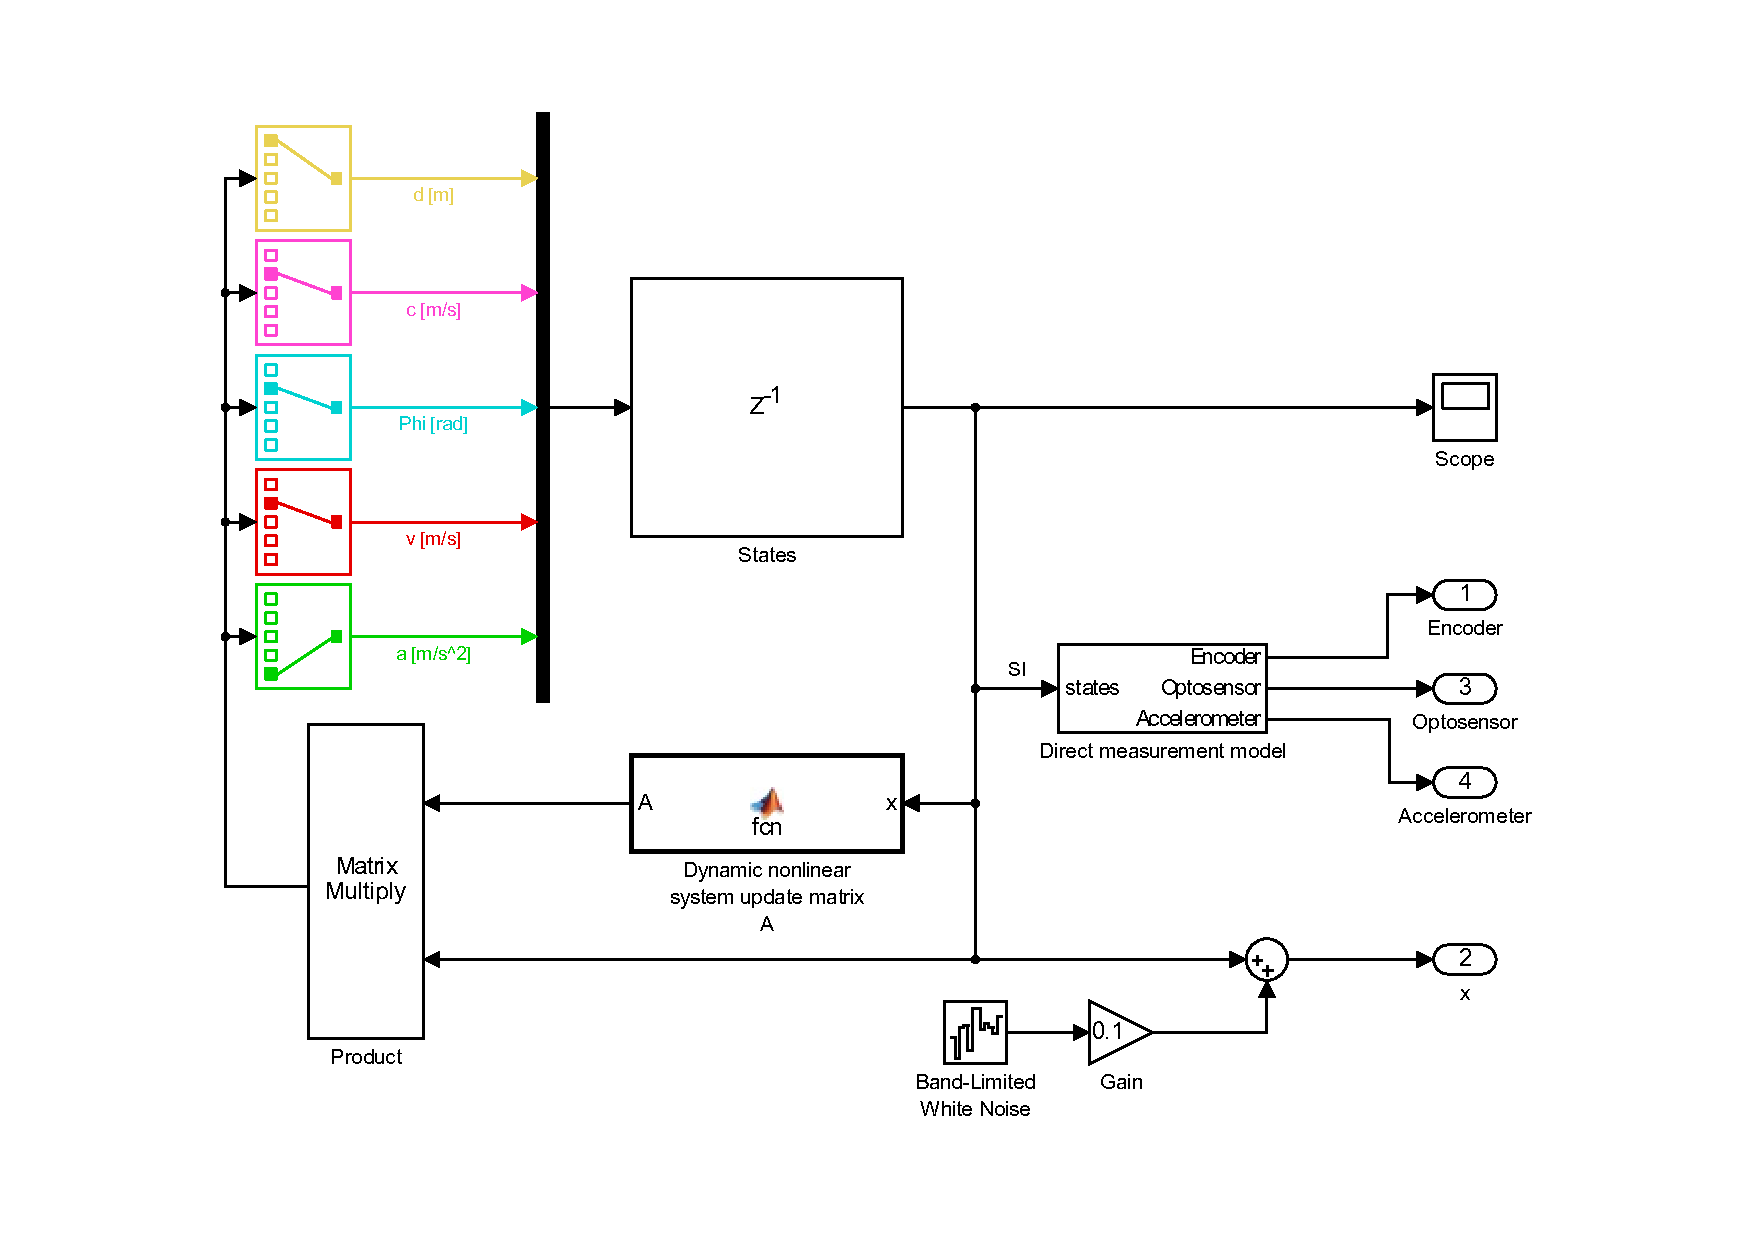
\includegraphics[width=0.7\linewidth]{img/sys}
    \centering
    \vspace{-20pt}
    \caption{Simulator model based on Jacobian matrices}
    \label{fig:model}
\end{figure}

The \textbf{Dynamic nonlinear system update matrix A} block contains a simple MATLAB script that builds the current system update matrix based on the Jacobian functions and the current states. Once we possess this, the system update phase can be executed just like in a linear case, with a matrix product. The resulting vector is the new set of state variables.

\subsection{Implementation of the control system}

To describe the implementation of the entire control system is out of the scope of this paper, however, key aspects of the software will be highlighted. The visual development of the software requires a different way of thinking than working with traditional source code. Therefore, we encourage the reader to design his or her own control system, in order to get a first hand experience in model based design.

\paragraph{Inverse measurement model}

The implementation of the inverse measurement model described earlier. During the race, multiple signals provide information about the track (optosensor array, side proximity sensors), therefore an inverse measurement model must be derived and realized for each of them, to provide the system states for the controller.

\paragraph{Controller}

Although basic processing might be required to enhance the raw signal quality before the inverse measurement model, any serious processing should be implemented in the next stage. Using model based design, several controller implementations can be evaluated quickly by testing and comparing them using the dynamic simulation of the model. A word of caution though: an inferior simulator can negatively influence the results of the comparison. Always introduce the major physical limitations to the system, for example the non-zero transition time of the steering servo between states.

\subsection{High level control, state machine}

\verb!MATLAB! has an extension called \verb!Stateflow! dedicated to the development of state machines. It integrates seamlessly with simulink models, and supports a wide range of features including subcharts, temporal logic and code generation as well, making it a very powerful tool. Figure \ref{fig:stateflow} shows the top layer of the state machine implementation of the obstacle course in \verb!Stateflow!. It is primarily used to detect certain sections during the race based on the external signals, and take over the control of the car at some points to perform an action like the automated parking.

\begin{figure}[!ht]
    \centering
    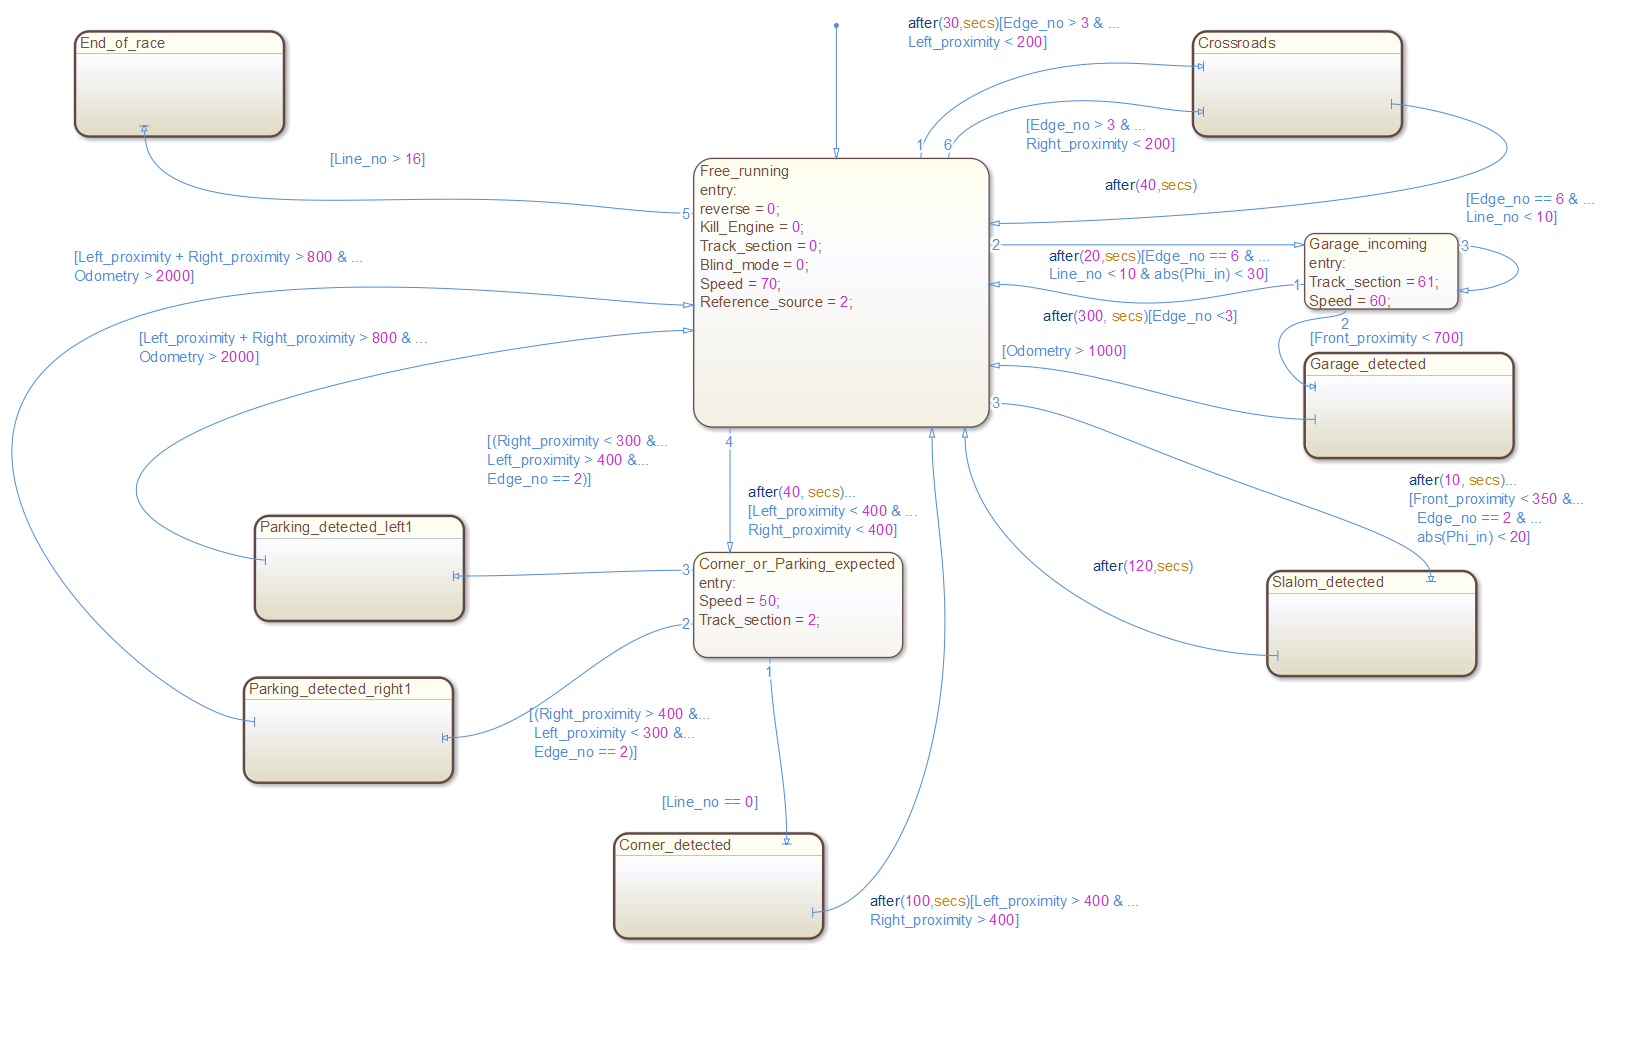
\includegraphics[width=0.7\linewidth]{img/stateflow}
    \centering
    \caption{State machine diagram of the obstacle course}
    \label{fig:stateflow}
\end{figure}





